%%%%%%%%%%%%%%%%%%%%%%%%%%%%%%%%%%%%%%%%%%%%%%%%%%%%%%%%%%%%%%%%%%%%
% PREAMBLE
%%%%%%%%%%%%%%%%%%%%%%%%%%%%%%%%%%%%%%%%%%%%%%%%%%%%%%%%%%%%%%%%%%%%

\documentclass[handout]{beamer}
%\documentclass{beamer}

%------------------------------------------------------------------
% Presentation Settings
%------------------------------------------------------------------

\mode<presentation>
{
	\usetheme{Boadilla}      % or Boadilla, Singapore, ...
	\usecolortheme{default} % or albatross, beaver, crane, ...
	\usefonttheme{default}  % or serif, structurebold, ...
	\setbeamertemplate{navigation symbols}{}
	\setbeamertemplate{caption}[numbered]
	\setbeamertemplate{itemize items}[circle]
	\setbeamertemplate{itemize subitem}[triangle]
	\setbeamertemplate{enumerate items}[default]
	\setbeamerfont{caption}{size=\tiny}
	%\setbeamercolor{alerted text}{fg=blue}
}

%------------------------------------------------------------------
% Packages
%------------------------------------------------------------------
\usepackage{amsmath}
\usepackage[natbibapa]{apacite}
\usepackage{appendixnumberbeamer}
\usepackage[english]{babel}
\usepackage{comment}
\usepackage{hyperref}
\usepackage[utf8x]{inputenc}
\usepackage{pdfpages}
\usepackage{subcaption}
\usepackage{verbatim}

\usepackage{listings} % Code blocks
\usepackage{color}

\definecolor{ltgreen}{RGB}{230, 242, 230}

\lstset{frame=tb,
  language=bash,
  aboveskip=3mm,
  belowskip=3mm,
  showstringspaces=false,
  columns=flexible,
  basicstyle={\small\ttfamily},
  numbers=none,
  breaklines=true,
  breakatwhitespace=true,
  tabsize=3,
  backgroundcolor=\color{ltgreen}
}


%------------------------------------------------------------------
% Set up
%------------------------------------------------------------------

% Add section titles

\AtBeginSection[]{
	\begin{frame}
  	\vfill
  	\centering
  	\begin{beamercolorbox}[sep=8pt,center,shadow=false,rounded=false]{title}
    	\usebeamerfont{title}\insertsectionhead\par%
  	\end{beamercolorbox}
  	\vfill
  \end{frame}
}

% Reduce references font size

\renewcommand*{\bibfont}{\scriptsize}

%------------------------------------------------------------------
% Title page settings
%------------------------------------------------------------------

\title[Git/GitHub Workshop: Part 3]{Workshop: Introduction to Git and GitHub}

\subtitle{Part 3: Git Branching}

\author[P. Joly]{Philippe Joly}
\institute[FU-Berlin]{Freie Universität Berlin}

\date{March 9, 2021}

%%%%%%%%%%%%%%%%%%%%%%%%%%%%%%%%%%%%%%%%%%%%%%%%%%%%%%%%%%%%%%%%%%%%
% DOCUMENT
%%%%%%%%%%%%%%%%%%%%%%%%%%%%%%%%%%%%%%%%%%%%%%%%%%%%%%%%%%%%%%%%%%%%

\begin{document}

%------------------------------------------------------------------
% Title Page
%------------------------------------------------------------------
\begin{frame}
\titlepage
\end{frame}
%

%\begin{columns}
%  \begin{column}{0.5\textwidth}
%
%    ...
%
%  \end{column}
%  \begin{column}{0.5\textwidth}
%    ...
%  \end{column}
%\end{columns}

%\begin{lstlisting}
%$ cd /home/user/my_project
%\end{lstlisting}

%\begin{figure}
%	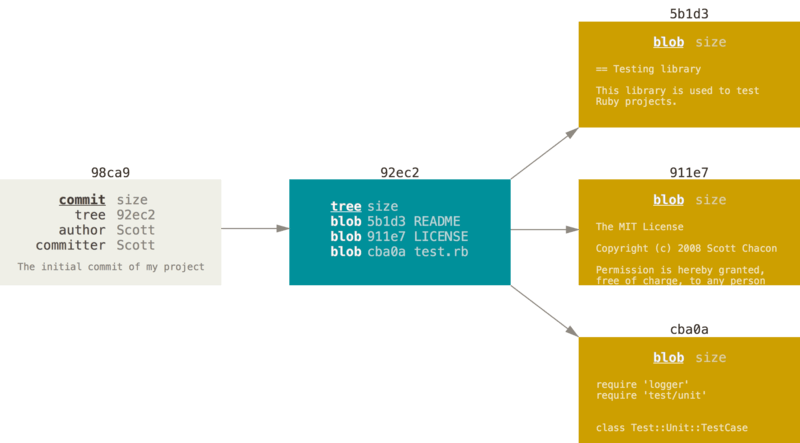
\includegraphics[width=0.9\textwidth]{figures/fig09_commit.png}
%	\caption{A commit and its tree. \textit{Source}: Chacon \& Straub (2021), fig. 9.}
%\end{figure}

%%------------------------------------------------------------------

\begin{frame}{Reference}
	\begin{columns}
	
		\begin{column}{0.5\textwidth}
			\begin{itemize}
				\item This workshop draws extensively on Scott Chacon and Ben Straub (2021), \href{https://git-scm.com/book/en/v2}{\textit{ProGit}}, Version 2.1.295, 2021-02-26. 
				\item Like the book, this workshop carries the CC BY-NC-SA 3.0 license.
			\end{itemize}
		\end{column}
		
		\begin{column}{0.5\textwidth}
			\begin{figure}
				
\includegraphics[width=0.5\textwidth]{figures/progit_cover.png}
				\caption{}
			\end{figure}
		\end{column}
	
	\end{columns}
\end{frame}

%%------------------------------------------------------------------

\begin{frame}{Git branching}
	\begin{itemize}
		\item A divergence from the main line of development
		\item Git “killer feature”
		\begin{itemize}
			\item Lightweight
			\item Fast
			\item Encourages workflows that branch and merge often
			\item Let's you freely experiment
			\item Structures collaboration
		\end{itemize}
	\end{itemize}
\end{frame}
	
\begin{frame}{A branch is simply a pointer}
\begin{figure}
	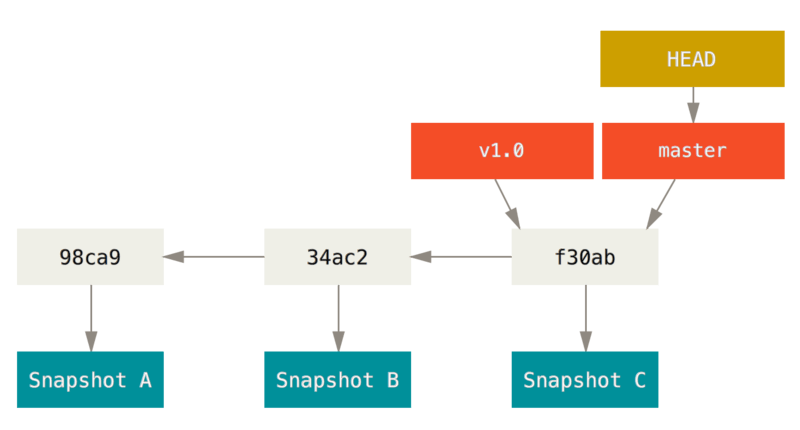
\includegraphics[width=0.9\textwidth]{figures/fig11_branch_history.png}
	\caption{A branch and its commit history. \textit{Source}: Chacon \& Straub (2021), fig. 11.}
\end{figure}
\end{frame}	

\begin{frame}[fragile]{Creating a branch adds a pointer to your commit history}
\begin{lstlisting}
$ git branch testing
\end{lstlisting}
\begin{figure}
	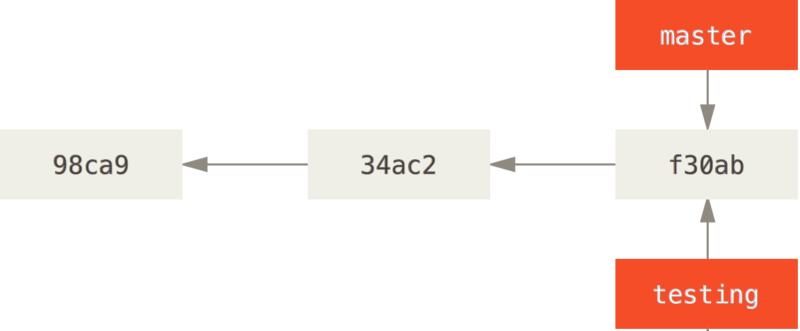
\includegraphics[width=0.9\textwidth]{figures/fig12_new_branch.png}
	\caption{Two branches pointing into the same series of commits. \textit{Source}: Chacon \& Straub (2021), fig. 12.}
\end{figure}
\end{frame}

\begin{frame}[fragile]{HEAD points to your current position}
\begin{lstlisting}
$ git branch
* master
  testing
\end{lstlisting}
\begin{figure}
	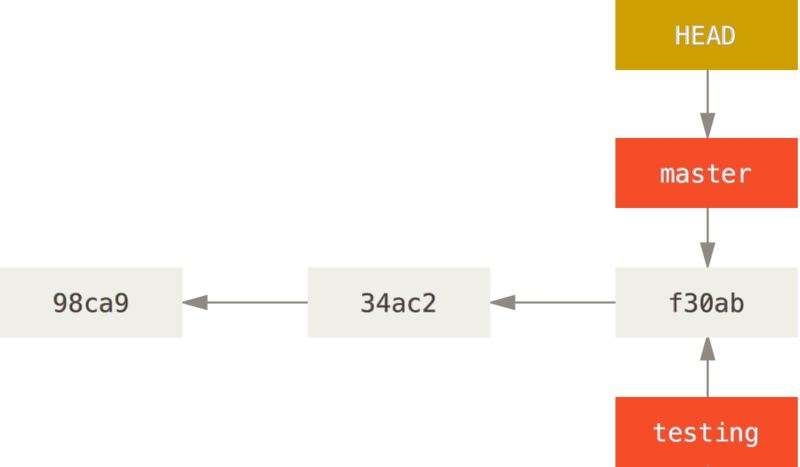
\includegraphics[width=0.8\textwidth]{figures/fig13_head.png}
	\caption{HEAD pointing to a branch. \textit{Source}: Chacon \& Straub (2021), fig. 13.}
\end{figure}
\end{frame}

\begin{frame}[fragile]{Switching branches}
\begin{lstlisting}
$ git checkout testing
$ git branch
  master
* testing
\end{lstlisting}
\begin{figure}
	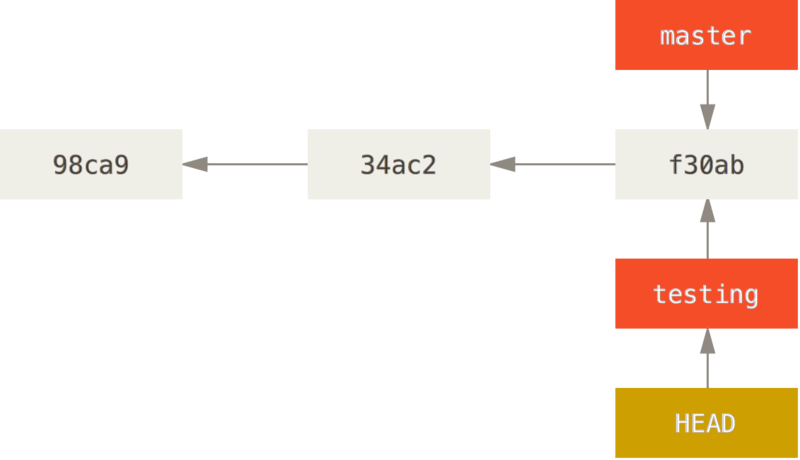
\includegraphics[width=0.7\textwidth]{figures/fig14_head_switch.png}
	\caption{HEAD points to the current branch. \textit{Source}: Chacon \& Straub (2021), fig. 14.}
\end{figure}
\end{frame}

\begin{frame}[fragile]{The \texttt{testing} (the new branch) moves forward}

\begin{lstlisting}
$ git add myfile.txt
$ git commit -m "add this new file"
\end{lstlisting}

\begin{figure}
	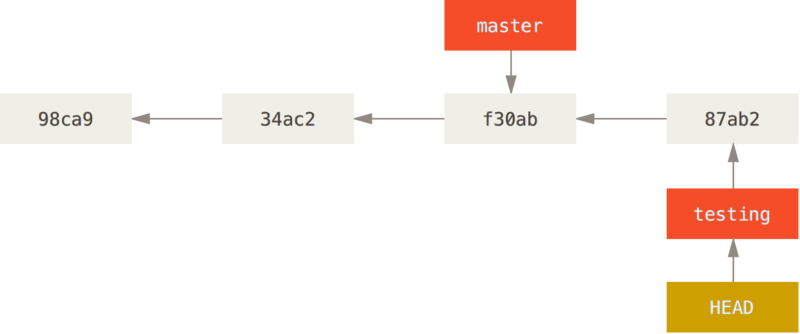
\includegraphics[width=0.9\textwidth]{figures/fig15_testing_forward.png}
	\caption{HEAD points to the current branch. \textit{Source}: Chacon \& Straub (2021), fig. 15.}
\end{figure}
\end{frame}


\begin{frame}[fragile]{Back to \texttt{master} (the main branch)}

\begin{lstlisting}
$ git checkout master
\end{lstlisting}

\begin{figure}
	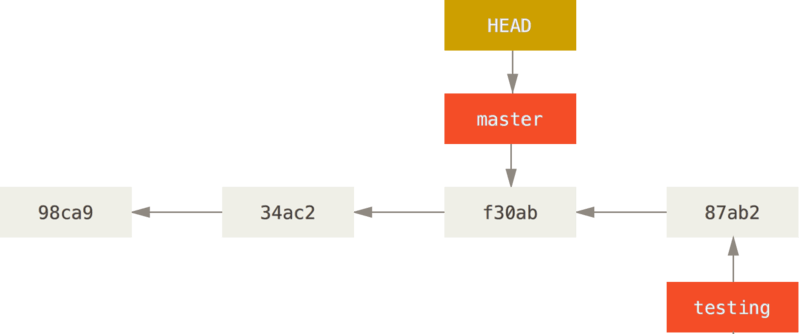
\includegraphics[width=0.9\textwidth]{figures/fig16_back_to_master.png}
	\caption{HEAD moves when you checkout. \textit{Source}: Chacon \& Straub (2021), fig. 16.}
\end{figure}
\end{frame}

\begin{frame}[fragile]{\texttt{master} moves forward: a divergent history}

\begin{lstlisting}
$ git add myfile2.txt
$ git commit -m "add another file"
\end{lstlisting}

\begin{figure}
	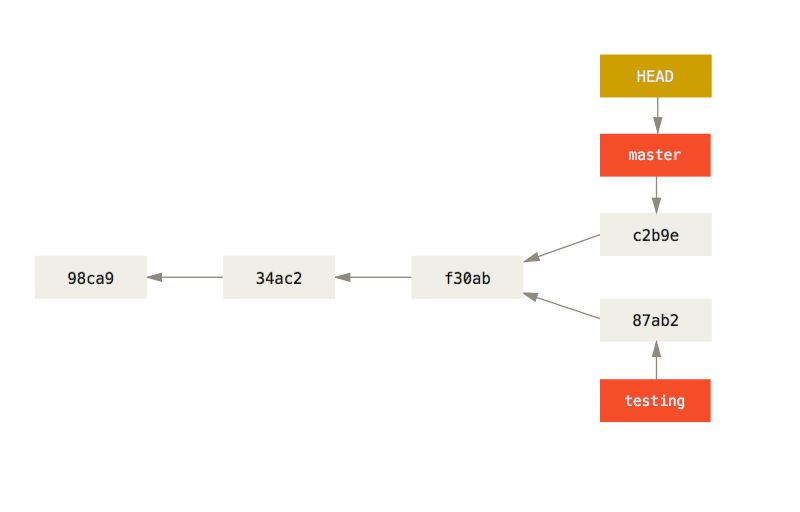
\includegraphics[width=0.7\textwidth]{figures/fig17_diverge.png}
	\caption{Divergent history. \textit{Source}: Chacon \& Straub (2021), fig. 17.}
\end{figure}
\end{frame}

\begin{frame}[fragile]{Creating and switching branches: summary}
Create a new branch
\begin{lstlisting}
$ git branch newbranch
\end{lstlisting}
Switch to that branch
\begin{lstlisting}
$ git checkout newbranch
\end{lstlisting}
Shortcut: create \textit{and} switch to a new branch 
\begin{lstlisting}
$ git checkout -b newbranch
\end{lstlisting}
List your branches and see on which one you are now
\begin{lstlisting}
$ git branch
\end{lstlisting}
\end{frame}

\begin{frame}{Basic merging (1)}
\begin{figure}
	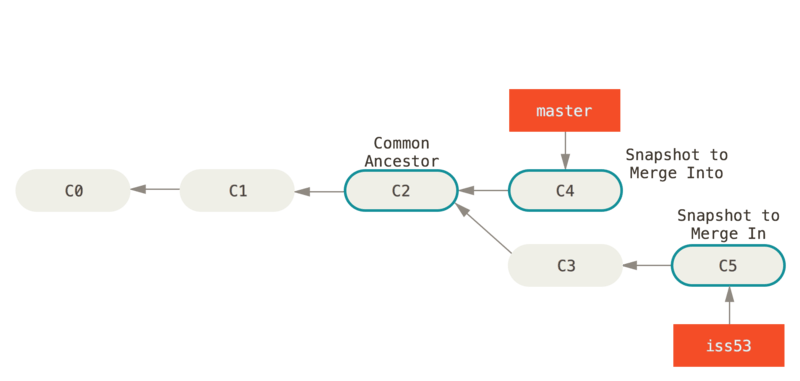
\includegraphics[width=0.9\textwidth]{figures/fig24_pre_merge.png}
	\caption{Three snapshots used in a typical merge. \textit{Source}: Chacon \& Straub (2021), fig. 24.}
\end{figure}
\end{frame}

\begin{frame}[fragile]{Basic merging (2)}
Move (\texttt{checkout}) to the \textbf{receiving} branch ({master}) before merging
\begin{lstlisting}
$ git checkout master
$ git merge iss53
\end{lstlisting}
\begin{figure}
	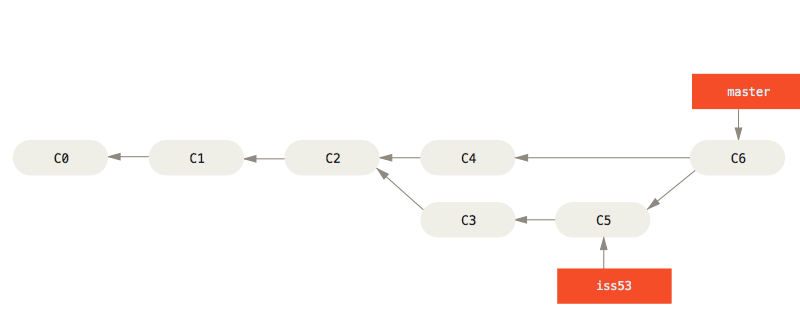
\includegraphics[width=0.9\textwidth]{figures/fig25_merge.png}
	\caption{A merge commit. \textit{Source}: Chacon \& Straub (2021), fig. 25.}
\end{figure}
\end{frame}

\begin{frame}[fragile]{Deleting a branch}
After merging, you can safely delete the branch. 
\begin{lstlisting}
$ git branch -d iss53
\end{lstlisting}
\end{frame}

\end{document}



